\subsection{Reactive Power} \label{subsec:ReactivePower}
If a voltage $v$ in $\phi = 0$ is applied across a pure reactance, as in eq \refq{eq:4_1_1_CapCurrent4}, it will cause the resulting current to be phase shifted by $\pm$\SIQ{90}{\degree}. This is shown in eq \ref{eq:4_1_1_ReactiveCurrentPhaseShift}. 
\begin{equation}\label{eq:4_1_1_ReactiveCurrentPhaseShift}
    i(\omega) = \frac{v(\omega)}{-\frac{j}{\omega C}} = v(\omega) \cdot j \omega C 
\end{equation}
The current is leading the voltage as shown in \ref{eq:4_1_1_ReactiveCurrentPhaseShift} and figure \ref{fig:4_1_1_ReactanceCurrentLeadVoltage}.
\begin{figure}[H]
    \centering
    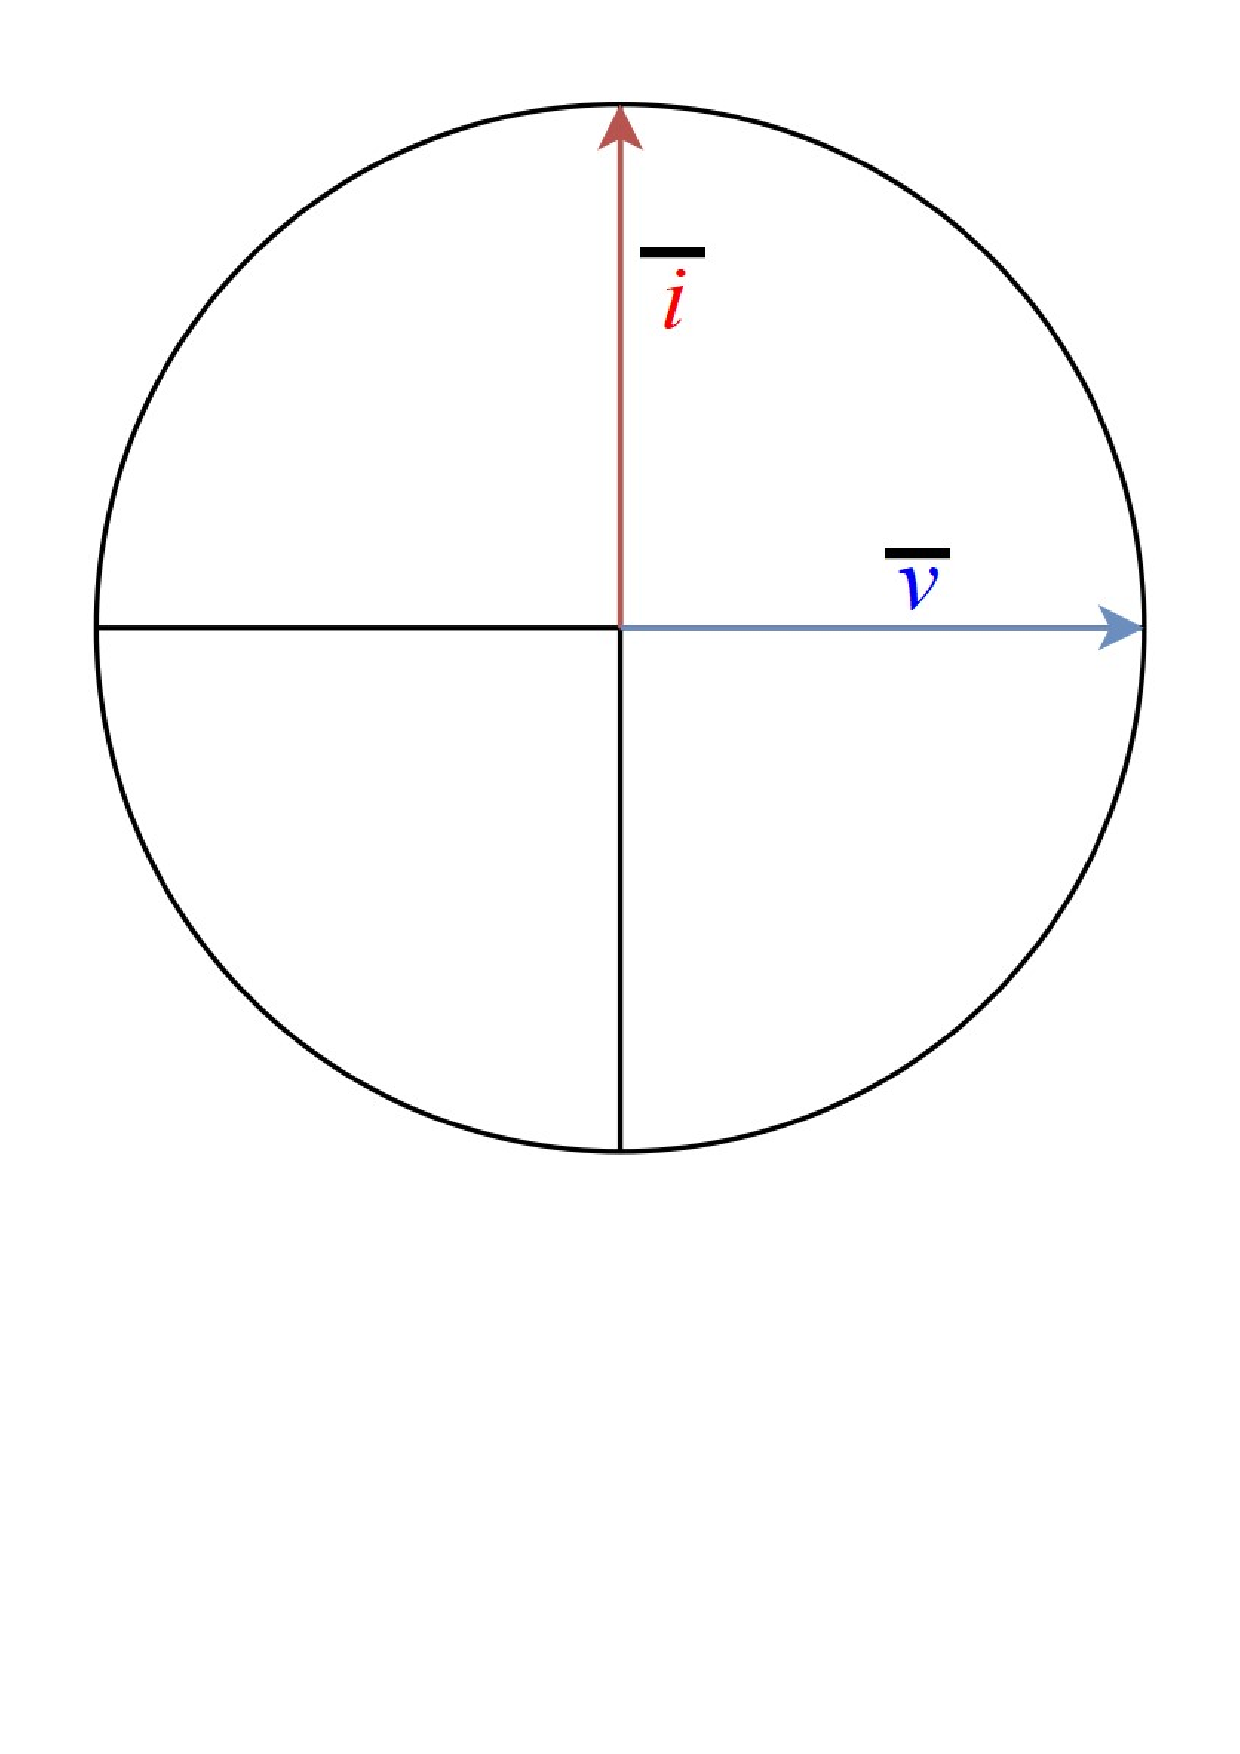
\includegraphics[clip, trim=0 250 0 0, width=0.4\textwidth]{Sections/4_TechnicalAnalysis/Figures/4_1_1_ReactanceCurrentPhase.pdf}
    \caption{The current is leading the voltage by \SIQ{90}{\degree} when a voltage is applied across the capacitive reactance.}
    \label{fig:4_1_1_ReactanceCurrentLeadVoltage}
\end{figure}

The power dissipated in the reactance is the vector product of the current and voltage as shown in equation \refq{eq:4_1_1_ReactivePowerLossLess}.
\begin{equation}\label{eq:4_1_1_ReactivePowerLossLess}
    P = \bar i \cdot \bar v = |\bar i| |\bar v| cos(\phi)
\end{equation}

Since $\phi = \frac{\pi}{2}$ (or \SIQ{90}{\degree}) then $cos(\pi/2) = 0$ and the power dissipated in the reactance is 0 as shown in eq \ref{eq:4_1_1_ReactivePowerLossLess2}
\begin{equation}\label{eq:4_1_1_ReactivePowerLossLess2}
    P = \bar i \cdot \bar v = |\bar i| |\bar v| cos\left(\frac{\pi}{2}\right) = 0
\end{equation}
This result means that an ideal capacitor with an impedance that is a pure reactance cannot dissipate any power. It is lossless. The same is true for inductors with the current vector lagging the voltage by \SIQ{90}{\degree}. Real components are not purely reactive however, they have resistance in the leads and materials used to construct them and the dieelectric material in a capacitor can absorb energy leading to losses. 
